\section{"Milestones" der Molekularbiologie/Genetik}
\txc{Füge ich nach, falls tatsächlich relevant.}

\section{Das zentrale Dogma der Molekularbiologie}

\begin{center}
    ``The central dogma states that information in nucleic acid can be perpetuated or transferred, but the transfer of
    information into protein is irreversible''
\end{center}

\begin{center}
    ``DNA macht RNA macht Protein''
\end{center}

\defin{dogma}

\begin{figure}[H]
    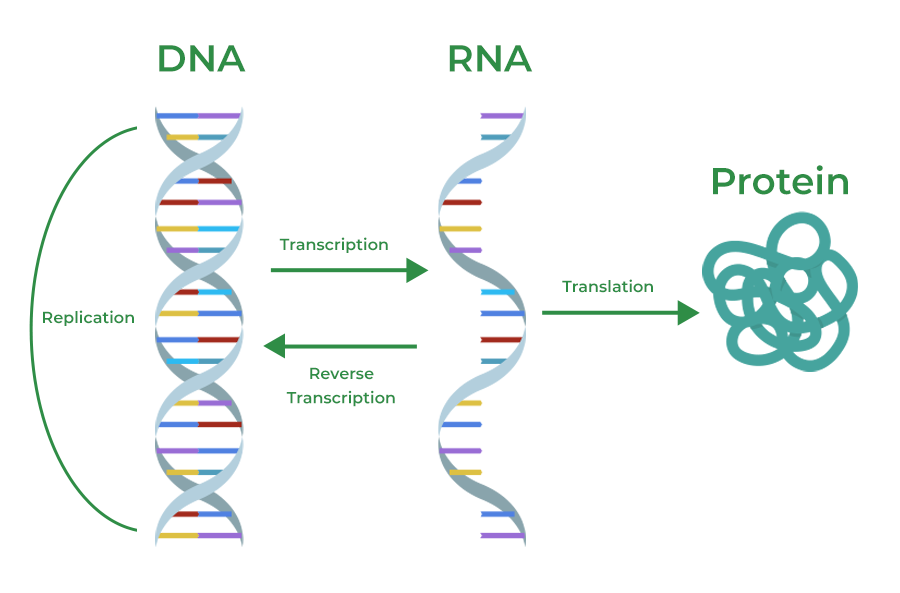
\includegraphics[width=\textwidth]{images/dogma}
    \caption{Code Sonne von \url{https://www.geeksforgeeks.org/biology/central-dogma-steps-guide/}}
\end{figure}


% TODO F 33- 35

\section{Der gentische Code}

\begin{figure}[H]
    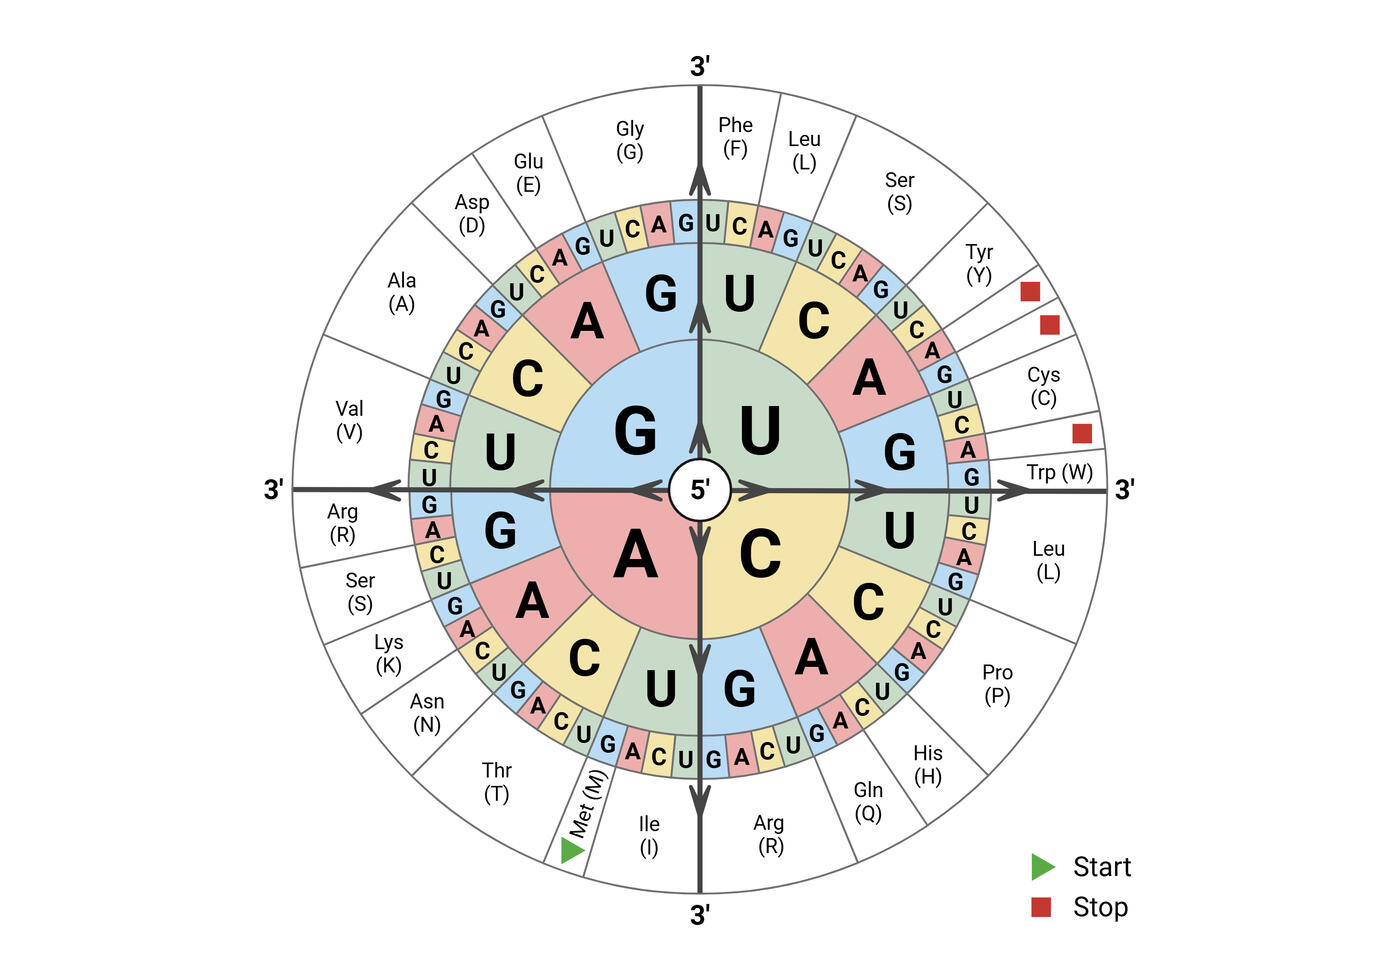
\includegraphics[width=\textwidth]{images/code_sonne}
    \caption{Code Sonne von \url{https://www.openscience.or.at/de/wissen/genetik-und-zellbiologie/2013-03-10-der-genetische-code/}}
\end{figure}

\section{Eukaryotisches "Muster-Gen"}

\begin{figure}[H]
    % TODO Bild
    \caption{Pol II}
\end{figure}


\section{Exons und Introns}

% TODO BILD

Gene mit drei Exons finden Sie in Lehrbüchern immer wieder, diese sind aber real eher selten.
Das ATG muss nicht im ersten Exon sein (und das ATG bestimmt KEINESFALLS den Anfang eines Exons)
